% --- Configuration ----------------------------------------------------

\documentclass[12pt,titlepage]{article}

\usepackage[utf8]{inputenc}

\usepackage{kpfonts}
\usepackage[T1]{fontenc}

% \usepackage{sansmathfonts}
% \usepackage[T1]{fontenc}
% \renewcommand*\familydefault{\sfdefault}

% \usepackage[T1]{fontenc}
% \usepackage[sfdefault]{FiraSans}
% \usepackage{newtxsf}

\usepackage{graphicx}
\graphicspath{ {./figures/} }

\usepackage[margin=1in]{geometry}

\usepackage{amsmath}

\usepackage{booktabs}

\usepackage{chngpage}

\usepackage{hyperref}
\hypersetup{colorlinks=True, citecolor=red, urlcolor=blue}

\usepackage{minted}

\usepackage{nomencl}
\makenomenclature

\usepackage{biblatex}
\addbibresource{references.bib}

% Run this command in the terminal to build the nomenclature then rerun latex
% makeindex main.nlo -s nomencl.ist -o main.nls

%--- Document ---------------------------------------------------------

\title{\textbf{BFB reactor model}}
\author{Gavin Wiggins and Cornelius Agu}
\date{\today}

\begin{document}

\maketitle

\tableofcontents

\section{Introduction}

This documentation is for the one-dimensional bubbling fluidized bed (BFB) reactor model developed in Python. The model predicts dynamic and steady-state conditions of a BFB reactor. See the sections below for installation and usage information along with discussions of the equations that are utilized by the model. The Python code for the model is open source and available on GitHub at \url{https://github.com/wigging/bfb-reactor}. An online version of this documentation is hosted at \url{https://gavinw.me/bfb-reactor/}. This work is inspired by the one-dimensional gasification model published by Agu et al. \cite{Agu-2019f}.

\section{Installation}

A recent version of Python 3 is needed to run the BFB reactor model. The following Python packages are also required: NumPy, SciPy, and Matplotlib. The \href{https://www.anaconda.com/products/individual}{Anaconda} distribution of Python is recommended for Mac, Linux, and Windows operating systems.

\section{Usage}

Use the commands shown below to run each model from the terminal.

\begin{minted}{bash}
# Run the dynamic model
$ python dynamic examples/params.json --run

# Plot results from the dynamic model
$ python dynamic examples/params.json -plot

# Run the steady-state model
$ python steady
\end{minted}

\section{Constants}

This section provides equations for the various constants calculated by the model. The dimensionless Archimedes number is calculated as shown in Equation \ref{eq:archimedes}.

\begin{equation}\label{eq:archimedes}
    Ar = \frac{d_p^3 \rho_g (\rho_p - \rho_g) g}{\mu^2}
\end{equation}

\section{Reactor configuration}

Inlet/outlet flows and geometry of the reactor applicable to the BFB model are shown in Figure \ref{fig:grid}. Fuel (feedstock) enters at the side of the reactor while the fluidization gas enters at the bottom of the reactor. Products leave at the top of the reactor. The following distance or height parameters from the reactor bottom are utilized by the model: overall reactor height ($H$), total fluidized bed height ($H_f$), static bed height ($H_{s}$), and distance to the fuel inlet ($H_{in}$). Also shown in Figure \ref{fig:grid} is the staggered grid used by the model for the solid and gas phases. Solid fuel particles are assumed to move in a downward direction while gas moves in an upward direction. Distance between node points on the grid is represented by $\Delta z$.

\begin{figure}[ht]
    \centering
    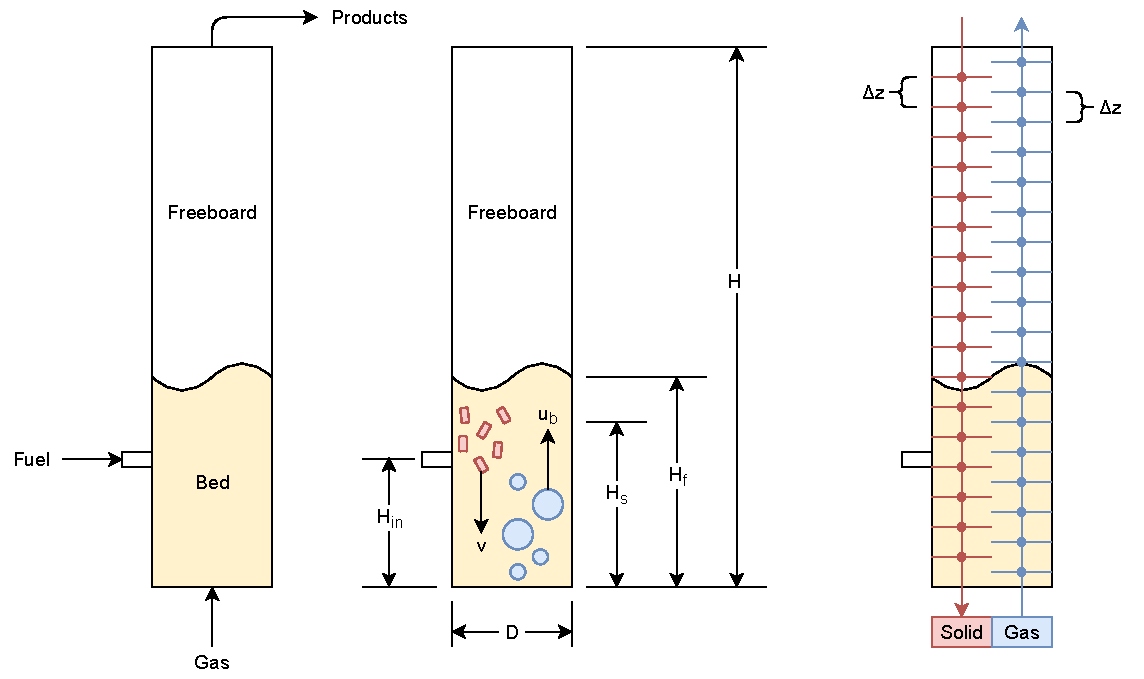
\includegraphics[width=0.8\textwidth]{figures/grid.pdf}
    \caption{Inlet and outlet flows (left), geometry parameters (center), and one-dimensional grid (right) for the BFB reactor model.}
    \label{fig:grid}
\end{figure}

\section{Reaction kinetics}

The kinetic scheme implemented by the model for biomass pyrolysis is shown in Figure \ref{fig:pyrolysis}. Biomass is the fuel (feedstock) fed to the reactor while volatiles, char, and tar are the pyrolysis products. The kinetic rate constant $k$ for each of the pyrolysis reactions are an Arrhenius form as depicted by Equation \ref{eq:kpyro}.

\begin{figure}[ht]
    \centering
    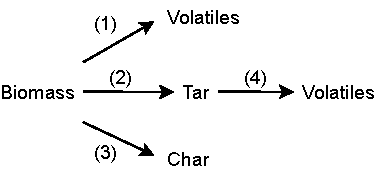
\includegraphics{figures/pyrolysis.pdf}
    \caption{Primary and secondary reactions for biomass pyrolysis.}
    \label{fig:pyrolysis}
\end{figure}

\begin{equation}
    k = A\; exp \left( -\frac{E}{R T} \right) \label{eq:kpyro}
\end{equation}

The steam-biomass gasification reactions and associated rate parameters are given below in Table \ref{tab:gasification}. Molar concentration is represented by [ ] in mol/m$^3$, pressure is $p$ in Pa, and $X_c$ is the char conversion factor. The reaction enthalpy is given as $\Delta H$ in kJ/mol and the rate constant $r$ is in mol/(m$^3 \cdot$s).

\begin{table}[ht]
    \caption{Steam-biomass gasification reactions and rate parameters.}
    \label{tab:gasification}
    \begin{adjustwidth}{-0.5in}{-0.5in}
    \centering
    \small
    \begin{tabular}{clllll}
        \toprule
        Item & Reaction & $\Delta$H & Rate constant & Ref. \\
        \midrule
        5 & C + H$_2$O $\rightarrow$ CO + H$_2$ & 131 & $\displaystyle r_5 = \frac{k_{5,1} x_{H_2O}}{1/p + k_{5,2} x_{H_2} + k_{5,3} x_{H_2O}} (1 - X_c) [C]$ & x \\[1.5em]
          & & & $\displaystyle k_{5,1} = 1.25 \times 10^5 exp\left( -\frac{28,000}{T} \right)$ & \\[1em]
          & & & $\displaystyle k_{5,2} = 3.26 \times 10^{-4}$ & \\[1em]
          & & & $\displaystyle k_{5,3} = 0.313 exp \left( -\frac{10,120}{T} \right)$ & \\[1em]
        6 & C + CO$_2$ $\rightarrow$ 2 CO & 172 & $\displaystyle r_6 = \frac{k_{6,1}}{1 + \frac{x_{CO}}{k_{6,2} x_{CO_2}}} [C]$ & x \\[1.5em]
          & & & $\displaystyle k_{6,1} = 3.6 \times 10^5 exp \left( -\frac{20,130}{T} \right)$ & \\[1em]
          & & & $\displaystyle k_{6,2} = 4.15 \times 10^3 exp \left( -\frac{11,420}{T} \right)$ & \\[1em]
        7 & C + 2H$_2$ $\rightarrow$ CH$_4$ & -75 & $\displaystyle r_7 = 6.11 \times 10^{-3} exp \left( -\frac{80,333}{R T} \right) [H_2][C]$ & x \\[1.5em]
        8 & CO + H$_2$O $\leftrightarrow$ CO$_2$ + H$_2$ & -41 & $\displaystyle r_8 = 0.278 exp \left(-\frac{12,560}{R T} \right) \left([H_2O][CO] - \frac{[H_2O][CO]}{k_8} \right)$ & x \\[1em]
          & & & $\displaystyle k_8 = 0.022 exp \left( \frac{34,730}{R T} \right)$ & \\[1em]
        9 & CH$_4$ + H$_2$O $\rightarrow$ CO + 3H$_2$ & 206 & $\displaystyle r_9 = 312 exp \left( -\frac{15,098}{T} \right) [CH_4]$ & x \\[1.5em]
        \bottomrule
    \end{tabular}
    \end{adjustwidth}
\end{table}

\section{Fluidization}

This section presents equations used to estimate the fluidized state of the BFB reactor. Equations are provided for the bed expansion and minimum fluidization velocity. The current version of the model neglects the effect of the unconverted fuel on the fluidization behavior.

\subsection{Minimum fluidization velocity}

The minimum fluidization velocity is determined by Equation \ref{eq:Umf} which relies on Equation \ref{eq:Umf-Re-mf} for the Reynolds number at minimum fluidization conditions \cite{Wen-1966}.

\begin{align}
    U_{mf} &= \frac{Re_{mf}\,\mu}{\rho_g d_p} \label{eq:Umf} \\
    Re_{mf} &= \sqrt{(33.7)^2 + 0.0408 Ar} - 33.7 \label{eq:Umf-Re-mf}
\end{align}

\subsection{Bed expansion}

The expanded bed height is estimated using several correlations as defined in this section. The correlations consider bubbling as well as slugging conditions that can occur in the reactor. Correlated parameters $a_b$ and $c_b$ for the bubbling regime are given below while the slugging regime is represented by $a_s$ and $c_s$. Notice that $\log$ represents the base $10$ logarithm \cite{Agu-2018}.

\begin{align}
    a_b &= \phi^{1.5} (4.168 - 1.389 \log(Ar))            & \log(Ar) < 3.5 \\
    a_b &= \phi^{1.5} (0.329 - 1.156\times10^3 Ar^{-0.9}) & \log(Ar) \geq 3.5\\
    c_b &= (1.321 + 8.161\times10^4 Ar^{-1.04})^{0.083}   & \log(Ar) > 0
\end{align}

\begin{align}
    a_s &= 0.725 + 0.230 \log(Ar)                     & \log(Ar) < 3.9 \\
    a_s &= 1.184 + 8.962\times10^4 Ar^{-1.35}         & \log(Ar) \geq 3.9 \\
    c_s &= 0.042 + 0.108 \log(Ar)                     & \log(Ar) < 4.0 \\
    c_s &= (0.978 - 1.964\times10^2 Ar^{-0.8})^{4.88} & \log(Ar) \geq 4.0
\end{align}

When calculating the expanded bed height, the maximum bubble diameter in the bed is restricted by the reactor's bed diameter. This is accounted for by the maximum bubbling diameter to bed diameter ratio at the transition to slugging defined by Equations \ref{eq:db-D-max} and \ref{eq:db-D-bs} where $c_t = c_b / c_s$ and $a_t = 1 / (a_s - a_b)$ \cite{Agu-2019g}.

\begin{align}
    \left( \frac{\overline{d}_b}{D} \right)_\text{max} &= \text{min} \left(1,\; \left( \frac{\overline{d}_b}{D} \right)_\text{bs} \right) \label{eq:db-D-max} \\
    \left( \frac{\overline{d}_b}{D} \right)_\text{bs} &= 0.848 \left( \frac{U_{mf} \phi^{0.35} c_t^{a_t}}{D} \right)^{0.66} \left[ 1 - c (\phi^{0.35} c_t^{a_t})^{a-1} \right]^{0.66} \label{eq:db-D-bs}
\end{align}

The bubble diameter to bed diameter ratios ($\overline{d}_b/D$) in Equations \ref{eq:db-D-1} and \ref{eq:db-D-2} are selected based on the Archimedes number \cite{Agu-2019a, Werther-1974}. Similarly, the minimum slugging velocity to fluidization ratios ($U_{ms}/U_{mf}$) in Equations \ref{eq:Ums-Umf-1} and \ref{eq:Ums-Umf-2} are also related to the Archimedes number \cite{Agu-2018, Shaul-2012}.

\begin{align}
    \frac{\overline{d}_b}{D} &= 0.848 \left(\frac{U_s}{D} \right)^{0.66} \left[1 - c \left(\frac{U_s}{U_{mf}} \right)^{a - 1} \right]^{0.66} \quad \text{for}\quad Ar > 400 \label{eq:db-D-1} \\
    \frac{\overline{d}_b}{D} &= \frac{5.64\times10^{-4}}{D\,H_{mf}} \left[1 + 27.2 (U_s - U_{mf}) \right]^{1/3} \left[(1 + 6.84 H_{mf})^{2.21} - 1 \right] \quad \text{for}\quad Ar < 400 \label{eq:db-D-2}
\end{align}

\begin{align}
    \frac{U_{ms}}{U_{mf}} &= 1 + 2.33 U_{mf}^{-0.027} \left(\phi^{0.35} c_t^{a_t}-1 \right) \left(\frac{H_0}{D} \right)^{-0.588} \quad \text{for}\quad Ar > 400 \label{eq:Ums-Umf-1} \\
    \frac{U_{ms}}{U_{mf}} &= \left(e^{-0.5405 \frac{H_0}{D}} \right) \left(\frac{4.294\times10^3}{Ar} + 1.1 \right) + 3.676\times10^2 Ar^{-1.5} + 1 \quad \text{for}\quad Ar < 400 \label{eq:Ums-Umf-2}
\end{align}

The total bed height is based on the bed expansion estimated from the fluidized height and the minimum fluidized height as depicted by Equation \ref{eq:delta-e} shown below. When $\overline{d}_b/D < (\overline{d}_b/D)_{max}$ then the bed expansion is calculated based on bubbling conditions using Equation \ref{eq:delta-e-bub}. During slugging conditions, the bed expansion considers the maximum height of the bed in terms of the bed expansion ratio $\Delta e_r$ as seen in Equation \ref{eq:delta-er} where the height ratios are given in Equations \ref{eq:h-ratio-1} and \ref{eq:h-ratio-2}. Finally, Equations \ref{eq:Hf}, \ref{eq:Hmf}, and \ref{eq:emf} are used to determine the total bed height during fluidization \cite{Agu-2019b, Agu-2019f, Agu-2019g, Wen-1966}.

\begin{equation} \label{eq:delta-e}
    \Delta e = \frac{H_f - H_{mf}}{H_{mf}} = \frac{H_f}{H_{mf}} - 1
\end{equation}

\begin{equation} \label{eq:delta-e-bub}
    \Delta e = \left[ 1 - 0.103 (U_s - U_{mf})^{-0.362} \left( \frac{\overline{d}_b}{D} \right) \right]^{-1} - 1
\end{equation}

\begin{equation} \label{eq:delta-er}
    \Delta e = \Delta e_r - 1 = \left(\frac{H_{max}}{H_{mf}}\right) \left(\frac{H_f}{H_{max}}\right) - 1
\end{equation}

\begin{align}
    \frac{H_{max}}{H_{mf}} &= \left[1 - 0.103 (U_{ms} - U_{mf})^{-0.362} \left( \frac{\overline{d}_b}{D} \right) \right]^{-1} \label{eq:h-ratio-1} \\
    \frac{H_{f}}{H_{max}} &= \left[1 - 0.305 (U_s - U_{mf})^{-0.362} D^{0.48} \right]^{-1} \label{eq:h-ratio-2}
\end{align}

\begin{align}
    H_f &= H_{mf} (\Delta e + 1) \label{eq:Hf} \\
    H_{mf} &= \frac{1 - \epsilon_0}{1 - \epsilon_{mf}} \; H_0 \label{eq:Hmf} \\
    \epsilon_{mf} = \left(\frac{0.071}{\phi}\right)^{1/3} &\quad \text{where} \quad \epsilon_{mf} = \text{max}(\epsilon_{mf},\; \epsilon_0) \label{eq:emf}
\end{align}

\subsection{Bubble characteristics}

Here for bubble rise velocity $u_B$ in ref Agu 2019b Equation 22.

Here for bubble volumetric flux $V_B$ in ref Agu 2018 Equation 17.

% --- Nomenclature -----------------------------------------------------

\nomenclature{$Ar$}{Archimedes number [-]}
\nomenclature{$D$}{bed diameter [m]}
\nomenclature{$d_p$}{bed particle diameter [m]}
\nomenclature{$H_0$}{initial or static bed height [m]}
\nomenclature{$H_f$}{total fluidized bed height [m]}
\nomenclature{$H_{mf}$}{bed height at minimum fluidization [m]}
\nomenclature{$Re$}{Reynolds number [-]}
\nomenclature{$U_{mf}$}{minimum fluidization velocity [m/s]}
\nomenclature{$U_{ms}$}{minimum slugging velocity [m/s]}
\nomenclature{$U_s$}{superficial gas velocity [m/s]}
\nomenclature{$\overline{d}_b$}{average bubble diameter [m]}
\nomenclature{$\Delta e$}{dimensionless bed expansion [-]}
\nomenclature{$\mu$}{dynamic gas viscosity [Pa$\cdot$s]}
\nomenclature{$\phi$}{bed particle sphericity [-]}
\nomenclature{$\epsilon_0$}{initial or static bed void fraction [-]}
\nomenclature{$\epsilon_{mf}$}{bed void fraction at minimum fluidization [-]}
\printnomenclature

% --- References -------------------------------------------------------

\printbibliography

\end{document}
